% Slide 19 — Evidência de heterogeneidade por perfil
\begin{frame}{Dominância depende do perfil operacional}
  \begin{columns}[T,onlytextwidth]
    \column{0.52\textwidth}
      \centering
      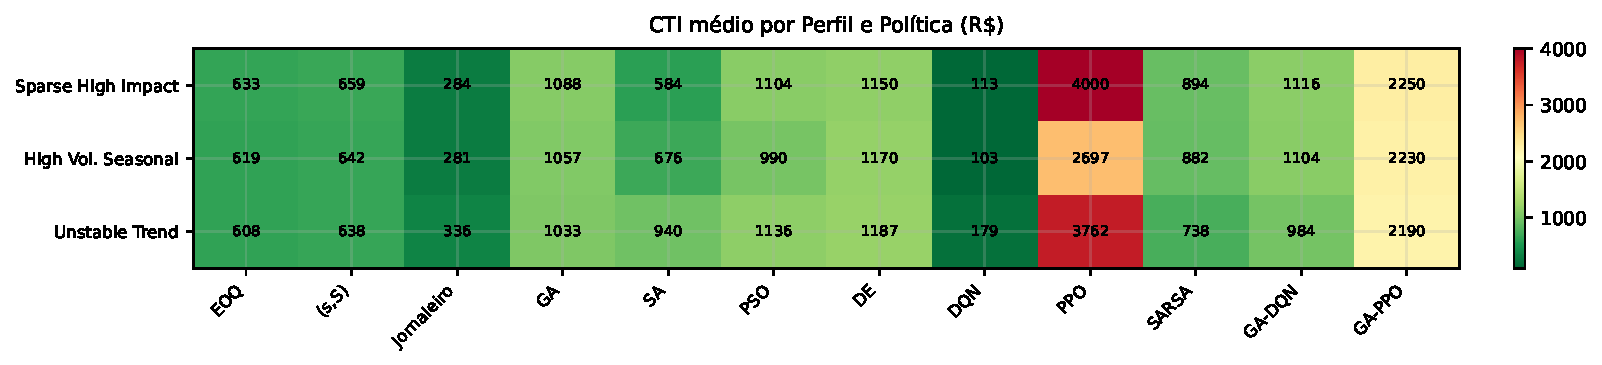
\includegraphics[width=\linewidth]{figures/profile_policy_heatmap_cti.pdf}\\
      \scriptsize CTI médio por política e POD
    \column{0.48\textwidth}
      \centering
      \resizebox{\linewidth}{!}{%
      \begin{tabular}{@{}lcrr@{}}
        \toprule
        \textbf{Perfil} & $n$ & \textbf{Dominante} & \textbf{CTI (R\$)} \\
        \midrule
        Sparse High Impact & 116 & SA & 584,01 \\
        Unstable Trend & 18* & EOQ & 607,95 \\
        High Vol. Seasonal & 11* & EOQ & 618,79 \\
        \bottomrule
      \end{tabular}}\\[0.4em]
      \scriptsize *$n<20$: evidência exploratória.
  \end{columns}
  \vspace{0.6em}
  \begin{alertblock}{Cuidado com o custo bruto}
    \small O Jornaleiro tem o \highlight{menor CTI bruto} em Sparse High
    Impact (R\$\,284), mas NS\,$=$\,0,55 -- abaixo do limiar de viabilidade
    de 0,70. Não é dominante: o ganho de custo não é alcançável sem violar
    o nível de serviço mínimo.
  \end{alertblock}
  \note{
    O heatmap mostra como o custo médio de cada política varia conforme o
    perfil operacional -- nenhuma célula é a mais clara em todas as linhas
    e colunas simultaneamente, o que é a evidência visual direta da
    heterogeneidade. A tabela à direita resume a política dominante por
    perfil, sempre sob a restrição de NS mínimo de 0,70: SA domina no
    perfil que concentra 80% das séries; EOQ domina nos dois perfis
    menores, que têm evidência exploratória por terem menos de 20 séries.
    É essencial destacar a ressalva do Jornaleiro: ele tem o menor custo
    bruto no perfil mais numeroso, mas seu nível de serviço de 0,55 está
    muito abaixo do limiar mínimo -- por isso ele é excluído da dominância,
    mesmo sendo o mais barato. Isso evita uma leitura simplista de que
    custo baixo implica política melhor.
  }
\end{frame}
